% Semantic search: the Python code of the Nordhjem search, step by step.
% Build from this folder:  tectonic semantic-search.tex
\documentclass[11pt]{article}
% Look and feel for the guides in this folder.
% Only the typeface block changes between design variants.

\usepackage{fontspec}
\usepackage[a4paper, left=2.7cm, textwidth=13.2cm, marginparsep=0.7cm,
  marginparwidth=4.0cm, top=3.0cm, bottom=3.2cm]{geometry}
\usepackage{xcolor}
\usepackage{booktabs}
\usepackage{tabularx}
\usepackage{amsmath}
\usepackage{amssymb}
\usepackage{enumitem}
\usepackage{listings}
\usepackage{tcolorbox}
\tcbuselibrary{skins}
\usepackage{marginnote}
\usepackage{tikz}
\usetikzlibrary{arrows.meta, positioning, calc, fit, shapes.geometric}
\usepackage{caption}
\usepackage{float}
\usepackage[hidelinks]{hyperref}

% ---- typeface (the design axis) -----------------------------------
\setmainfont{lmroman10}[Extension=.otf, UprightFont=*-regular, BoldFont=*-bold, ItalicFont=*-italic, BoldItalicFont=*-bolditalic]
\newcommand{\fontlabel}{Latin Modern Roman}

\setsansfont{texgyreheros}[Extension=.otf, UprightFont=*-regular,
  BoldFont=*-bold, ItalicFont=*-italic, BoldItalicFont=*-bolditalic,
  Scale=0.88]
\setmonofont{lmmono10}[Extension=.otf, UprightFont=*-regular,
  Scale=0.92]

% ---- colours: calm neutrals, one accent ----------------------------
\definecolor{ink}{HTML}{2E2622}
\definecolor{muted}{HTML}{7A6D64}
\definecolor{line}{HTML}{DDD3C7}
\definecolor{paper}{HTML}{F6F1EA}
\definecolor{accent}{HTML}{B5583A}
\definecolor{accentbg}{HTML}{F5E6DF}

\color{ink}
\linespread{1.12}
\setlength{\parindent}{1.2em}
\setlength{\parskip}{0pt}
\emergencystretch=3em
\frenchspacing

% ---- headings ------------------------------------------------------
\makeatletter
\renewcommand\section{\@startsection{section}{1}{0pt}%
  {3.2ex plus 1ex minus .2ex}{1.6ex}%
  {\normalfont\Large\color{ink}}}
\renewcommand\subsection{\@startsection{subsection}{2}{0pt}%
  {2.6ex plus .8ex minus .2ex}{1.0ex}%
  {\normalfont\large\itshape\color{ink}}}
\renewcommand\@seccntformat[1]{%
  \llap{\color{accent}\csname the#1\endcsname\hspace{0.9em}}}
\makeatother

% ---- running head and foot ----------------------------------------
\usepackage{fancyhdr}
\pagestyle{fancy}
\fancyhf{}
\renewcommand{\headrulewidth}{0pt}
\fancyhead[L]{\footnotesize\scshape\color{muted}%
  \MakeLowercase{Semantic search}}
\fancyhead[R]{\footnotesize\color{muted}\thepage}
\fancyheadoffset[R]{0pt}

% ---- margin notes: a short explanation of a term ------------------
\newcommand{\term}[2]{\emph{#1}\marginnote{\footnotesize\raggedright
  \color{muted}\textbf{\color{ink}#1:} #2}}
\renewcommand{\marginfont}{\footnotesize}

% ---- boxes ---------------------------------------------------------
\newtcolorbox{keypoint}{colback=accentbg, colframe=accentbg,
  boxrule=0pt, arc=0pt, left=10pt, right=10pt, top=7pt, bottom=7pt,
  borderline west={2pt}{0pt}{accent}}
\newtcolorbox{example}[1]{colback=white, colframe=line, boxrule=0.5pt,
  arc=0pt, left=10pt, right=10pt, top=6pt, bottom=6pt,
  fonttitle=\small\scshape, coltitle=muted, colbacktitle=white,
  title={\MakeLowercase{#1}}, titlerule=0.4pt, titlerule style=line}

% ---- code ----------------------------------------------------------
\lstset{
  basicstyle=\ttfamily\small,
  backgroundcolor=\color{paper},
  frame=none,
  xleftmargin=0.7em, xrightmargin=0.7em,
  aboveskip=0.9em, belowskip=0.9em,
  columns=fullflexible, keepspaces=true,
  showstringspaces=false,
  keywordstyle=\color{accent},
  commentstyle=\color{muted}\itshape,
  literate={×}{{$\times$}}1 {→}{{$\rightarrow$}}1
           {æ}{{\ae}}1 {ø}{{\o}}1 {å}{{\aa}}1 {ü}{{\"u}}1
}
\newcommand{\code}[1]{\texttt{#1}}

% ---- captions and tables -------------------------------------------
\captionsetup{font={small}, labelfont={sc,color=muted},
  textfont={color=muted}, labelsep=quad, justification=raggedright,
  singlelinecheck=false}
\renewcommand{\arraystretch}{1.18}

% ---- figure styles -------------------------------------------------
\tikzset{
  box/.style={draw=line, fill=white, rounded corners=3pt,
    font=\small, align=center, inner sep=6pt, minimum height=8mm},
  hot/.style={box, draw=accent, fill=accentbg},
  flow/.style={-{Stealth[length=2.2mm]}, draw=muted, line width=0.6pt},
  hotflow/.style={-{Stealth[length=2.2mm]}, draw=accent,
    line width=0.8pt},
  lbl/.style={font=\footnotesize, text=muted, align=center},
}

\raggedbottom


\begin{document}

% ---- title block ---------------------------------------------------
\thispagestyle{empty}
\setlength{\parindent}{0pt}
\vspace*{1.2cm}
{\color{muted}\scshape\MakeLowercase{Nordhjem store}
  \textperiodcentered{} \MakeLowercase{Guide}}\par
\vspace{0.9cm}
{\fontsize{28}{32}\selectfont Semantic search\par}
\vspace{0.5cm}
{\large\itshape\color{muted} The Python code behind the search box,\\
  one function at a time\par}
\vspace{0.6cm}
{\color{accent}\rule{2.2cm}{1.2pt}}\par
\vspace{0.6cm}
\begin{minipage}{11.5cm}
\small\color{muted}
This guide walks through the search as it is now in the repository:
\code{api/models.py}, \code{api/search.py} and
\code{api/parse\_query.py}. Every code block is the real code, and every
number was measured on the shop's 500 products. Section 1 explains
the ideas without code; the rest follows the code, one function at a
time.
\end{minipage}
\vspace{1.0cm}

{\small
\renewcommand{\contentsname}{\normalsize\scshape\color{muted}
  \MakeLowercase{Contents}}
\tableofcontents}

\newpage
\setlength{\parindent}{1.2em}

% ====================================================================
\section{What semantic search is}
\label{sec:ideas}

\subsection{The problem with matching words}

The simplest search compares \emph{words}. It counts how many words of
the question appear in each product's text, and shows the products
with the most. This is a \term{keyword search}{a search that matches
the letters of words, not what they mean.}. The shop started with one,
in \code{api/keyword\_search.py}.

Here it is on a real question:
\begin{quote}\itshape
a couch my guests can sleep on
\end{quote}

\begin{table}[H]
\small
\begin{tabularx}{\textwidth}{@{}l X l@{}}
\toprule
Rank & Product & Shared words \\
\midrule
1 & KILSHOLM sofa (a sofa bed) & a, guests, \ldots \\
2 & EGEEVIG sofa (a sofa bed) & a, guests, \ldots \\
3 & \textcolor{accent}{LUNDSTED rug} & \textcolor{accent}{a, can, on} \\
\bottomrule
\end{tabularx}
\caption{The keyword search. A rug comes third, because its text
``\ldots\ can be used outdoors on a terrace'' shares three small words
with the question.}
\end{table}

Two things go wrong. The word that matters, ``couch'', is in no product
text at all: the shop says ``sofa''. And small words such as ``a'',
``can'' and ``on'' count as much as the important ones. A keyword
search sees spelling. It does not see meaning.

\subsection{Searching by meaning}

\term{Semantic search}{a search that finds texts with the same
meaning, even when they use different words.} compares what the
question \emph{means} with what each product \emph{is}. ``couch'' and
``sofa'' mean the same thing; ``my guests can sleep on'' means ``folds
out into a bed for guests''. A semantic search finds the sofa beds, and
the rug drops to the bottom.

It needs a way to put meaning into a form a computer can compare. That
form is a list of numbers.

\subsection{Meaning as a list of numbers}

An \term{embedding model}{a model trained on huge amounts of text to
turn any text into a list of numbers, so that similar meanings give
similar numbers.} reads a text and returns a fixed-length list of
numbers. Here the model is Google's \code{gemini-embedding-001}, and
the list has 768 numbers. Such a list is called a \emph{vector}, and
the list for a text is its \emph{embedding}.

No single number means ``sofa'' or ``soft''. What matters is the whole
list, seen as a point in space. A map is a good picture: a city's
position takes two numbers, latitude and longitude, and cities close on
the map have close numbers. An embedding is a position with 768
numbers instead of 2, and texts with close meanings get close
positions. ``couch for guests'', ``sofa bed'' and ``Schlafsofa'' land
near each other; ``wool rug'' lands far away.

\subsection{Closeness as a score}

To compare two positions, the search measures the \emph{angle} between
the two vectors, as seen from zero. Pointing the same way means the
same meaning. This is the \term{cosine similarity}{a number for how
closely two vectors point the same way: 1 is the same direction, 0 is
unrelated.}: a score near 1 is close, lower is further.

When every vector is first scaled to length~1 (\emph{normalised}), the
cosine is simply the dot product: multiply the two lists pair by pair
and add up. That is one line of NumPy, \code{@}.

\subsection{How it works: two phases}

A semantic search is split into work done once, in advance, and work
done on every search.

\begin{figure}[H]
\centering
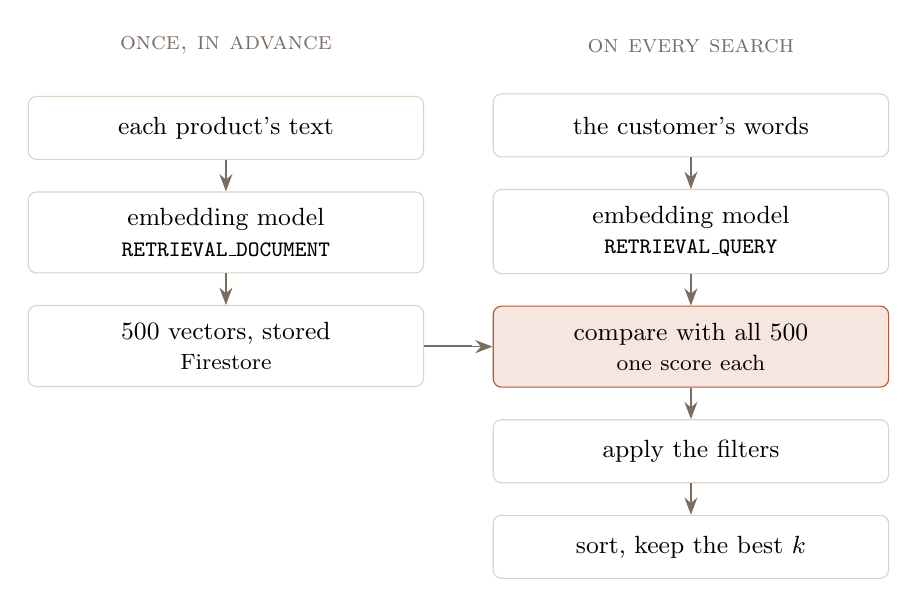
\begin{tikzpicture}[node distance=4mm and 7mm]
  \node[lbl, font=\small\scshape] (h1) {\MakeLowercase{Once, in advance}};
  \node[box, below=of h1, text width=46mm] (a1) {each product's text};
  \node[box, below=of a1, text width=46mm] (a2)
    {embedding model\\ \footnotesize \code{RETRIEVAL\_DOCUMENT}};
  \node[box, below=of a2, text width=46mm] (a3)
    {500 vectors, stored\\ \footnotesize Firestore};
  \draw[flow] (a1) -- (a2);
  \draw[flow] (a2) -- (a3);

  \node[lbl, font=\small\scshape, right=30mm of h1] (h2)
    {\MakeLowercase{On every search}};
  \node[box, below=of h2, text width=46mm] (b1) {the customer's words};
  \node[box, below=of b1, text width=46mm] (b2)
    {embedding model\\ \footnotesize \code{RETRIEVAL\_QUERY}};
  \node[hot, below=of b2, text width=46mm] (b3)
    {compare with all 500\\ \footnotesize one score each};
  \node[box, below=of b3, text width=46mm] (b4)
    {apply the filters};
  \node[box, below=of b4, text width=46mm] (b5)
    {sort, keep the best $k$};
  \draw[flow] (b1) -- (b2);
  \draw[flow] (b2) -- (b3);
  \draw[flow] (b3) -- (b4);
  \draw[flow] (b4) -- (b5);
  \draw[flow] (a3.east) -| ++(6mm,0) |- (b3.west);
\end{tikzpicture}
\caption{The two phases. The products are embedded once; only the
question is embedded on each search.}
\end{figure}

\paragraph{Once, in advance (\emph{indexing}).} Every product's text is
sent to the embedding model, and the 500 vectors are stored. This is
slow and costs a little money, so it happens once, and again only when
a product changes.

\paragraph{On every search (\emph{querying}).} Five steps:
\begin{enumerate}[leftmargin=1.6em, itemsep=2pt]
\item \textbf{Embed the question}: the customer's words become one
  vector, with the same model, so it lands in the same space as the
  products.
\item \textbf{Normalise} it to length~1, like the stored products.
\item \textbf{Score}: compare the question with every product; each
  gets one cosine score.
\item \textbf{Filter}: remove products that break a hard rule (wrong
  category, too expensive, wrong colour).
\item \textbf{Rank}: sort by score and return the best $k$ (the
  \emph{top-k}).
\end{enumerate}

\subsection{Meaning and rules}

Some wishes are about meaning: ``comfy'', ``for guests'', ``survives a
dog''. Others are rules with a yes or no answer: ``a sofa'', ``green'',
``under 3000~kr''. An embedding is good at the first kind and bad at
the second: it cannot tell that 8\,969 is more than 4\,000. So the
search uses both:

\begin{table}[H]
\small
\begin{tabularx}{\textwidth}{@{}l X X@{}}
\toprule
 & Meaning & Rules \\
\midrule
Example & comfy, for guests, cosy & sofa, dark green, at most 3000~kr \\
Handled by & the embedding: it \emph{ranks} & a filter: it
  \emph{removes} \\
Answer & a score, more or less & yes or no \\
In the code & \code{index.vectors @ question} & \code{filter\_products} \\
\bottomrule
\end{tabularx}
\caption{Two kinds of wish, two tools.}
\end{table}

Rules can come from a click (the Sofa chip, the price menu) or from the
words themselves (``under 3000''). Reading them from the words needs a
second, different model: a text model that fills in a form
(section~\ref{sec:words}).

\subsection{The words used in this guide}

\begin{table}[H]
\small
\begin{tabularx}{\textwidth}{@{}l X@{}}
\toprule
Word & Meaning here \\
\midrule
embedding, vector & the 768 numbers that stand for a text's meaning \\
embedding model & the model that makes them (\code{gemini-embedding-001}) \\
text model & a model that reads and writes text (\code{gemini-3-flash-preview}) \\
normalise & scale a vector to length 1, keeping its direction \\
cosine similarity, score & how close two meanings are; higher is closer \\
task type & a hint to the embedding model: question or document \\
index & all product vectors and fields, in memory, ready to compare \\
filter, mask & a rule; the True/False list that applies it \\
top-k & the $k$ best products, best first \\
structured output & a text model filling in a form instead of writing
  prose \\
hit@5, precision@5 & how the search is measured (section~\ref{sec:measure}) \\
\bottomrule
\end{tabularx}
\end{table}

\subsection{From ideas to code}

Each step is one Python function:

\begin{table}[H]
\small
\begin{tabularx}{\textwidth}{@{}X l l@{}}
\toprule
Step & Function & Section \\
\midrule
store the products (done once) & \code{loaders/load\_products.py} &
  \ref{sec:data} \\
read them into memory & \code{load\_index} & \ref{sec:index} \\
embed the question & \code{get\_embed\_query} & \ref{sec:question} \\
normalise & \code{normalise} & \ref{sec:question} \\
score & \code{index.vectors @ question} & \ref{sec:score} \\
filter & \code{filter\_products}, \code{np.where} & \ref{sec:filters},
  \ref{sec:search} \\
rank & \code{get\_top\_k} & \ref{sec:search} \\
all of it, in order & \code{search} & \ref{sec:search} \\
read rules from the words & \code{parse\_query}, \code{merge\_filters} &
  \ref{sec:words} \\
\bottomrule
\end{tabularx}
\end{table}

The rest of the guide follows that order, with the real code and real
numbers. Two searches are followed throughout: ``a couch my guests can
sleep on'' and ``green sofa that is comfy, less than 3000''.

% ====================================================================
\section{The data: products as numbers}
\label{sec:data}

\subsection{One product}

The shop has 500 products in \code{data/products.jsonl}, one per line.
Here is the first one, shortened:
\begin{lstlisting}
{"product_id": "P1001", "name": "KILGAARD mattress",
 "category": "mattress", "colour": "grey", "price_dkk": 1489.0,
 "description": "Memory foam mattress with medium firmness,
                 180x200 cm. Cooling cover that keeps you from
                 getting too warm at night."}
\end{lstlisting}

\subsection{Turning text into numbers}

A computer cannot compare meanings directly. So each product's text is
turned into an \term{embedding}{a list of numbers that stands for the
meaning of a text. Texts with similar meaning get similar lists.}: a
list of 768 numbers. The model that does this is
\code{gemini-embedding-001}, run on Google Cloud.

This happened \emph{once}, before any search, in
\code{loaders/load\_products.py}. For each product it builds one
sentence from the name, category, colour and description, and embeds
it:
\begin{lstlisting}[language=Python]
return (f"{product['name']}. Category: {category}. "
        f"Colour: {product['colour']}. {product['description']}")
\end{lstlisting}
The 500 lists of numbers are stored in Firestore, the shop's database,
in the collection \code{products}, one document per product, in a
field called \code{embedding}.

\subsection{Two kinds of text}

The loader embeds products with the task type
\code{RETRIEVAL\_DOCUMENT}; the search embeds the customer's words with
\code{RETRIEVAL\_QUERY}. A \term{task type}{a hint to the embedding
model about what the text is for, so it can place it better.} tells the
model which side of the search the text is on: a product
\emph{describes a thing}, a question \emph{describes a need}. Using the
query type for questions was measured on the 20 test questions:

\begin{table}[H]
\small
\begin{tabularx}{\textwidth}{@{}X r r@{}}
\toprule
Questions embedded as & precision@5 & gap to the first wrong product \\
\midrule
\code{RETRIEVAL\_QUERY} (used) & \textcolor{accent}{0.98} & +0.043 \\
\code{RETRIEVAL\_DOCUMENT} & 0.90 & +0.021 \\
\bottomrule
\end{tabularx}
\caption{The right task type finds more right products, and separates
them better from the wrong ones.}
\end{table}

% ====================================================================
\section{The index: all products in memory}
\label{sec:index}

\subsection{The \code{Index} class}

The search needs five things about every product: its ID, its numbers,
its category, its colour and its price. They are kept together in one
\term{dataclass}{a Python class that only holds values; Python writes
the \code{\_\_init\_\_} for you.}:
\begin{lstlisting}[language=Python]
@dataclass
class Index:
    """The products as NumPy arrays; row i of every array is product i."""

    ids: list[str]
    vectors: np.ndarray      # shape (n, 768), every row length 1
    categories: np.ndarray   # shape (n,), text
    colours: np.ndarray      # shape (n,), text
    prices: np.ndarray       # shape (n,), DKK
\end{lstlisting}
The rule that holds it together is in the docstring: \emph{row~i of
every array is product~i}. If \code{ids[7]} is \code{"P1008"}, then
\code{vectors[7]} are its numbers, \code{categories[7]} its category,
and so on. Every step later relies on that.

\code{Index} is the \emph{class}, the blueprint. \code{index =
Index(...)} makes one \emph{instance}, filled with real values. You
read from the instance: \code{index.prices}, never
\code{Index.prices}.

\subsection{\code{load\_index}: reading Firestore once}

\begin{lstlisting}[language=Python]
@lru_cache(maxsize=1)
def load_index() -> Index:
    db = firestore.Client(project=PROJECT)
    idd, vector, category, price, colour = [], [], [], [], []
    for document in db.collection("products").stream():
        product = document.to_dict()
        idd.append(document.id)
        vector.append(list(product["embedding"]))
        category.append(product["category"])
        price.append(product["price_dkk"])
        colour.append(product["colour"])
    store_index = Index(ids=idd, vectors=np.array(vector),
                        categories=np.array(category),
                        prices=np.array(price),
                        colours=np.array(colour))
    return store_index
\end{lstlisting}

Line by line:
\begin{itemize}[leftmargin=1.4em, itemsep=2pt]
\item \code{db.collection("products").stream()} hands over the 500
  documents one at a time.
\item \code{document.to\_dict()} turns one document into a Python
  dictionary, so \code{product["category"]} works.
\item Each field goes into its own list. Because all five lists grow
  together, row~i stays product~i.
\item \code{np.array(vector)} turns the list of 500 lists into one
  table of 500 rows and 768 columns. That is 3~MB in memory.
\end{itemize}

\term{\code{@lru\_cache}}{remembers what a function returned. The next
call with the same arguments returns the saved result without running
the function.} makes this run only on the first search. Reading
Firestore takes a few seconds; after that, every search reuses the same
\code{Index}.

\begin{keypoint}
The field names in Firestore come from the data, not from your code.
The data says \code{"colour"} (British spelling), so
\code{product["color"]} raises a \code{KeyError}, whatever you call your
own variables.
\end{keypoint}

% ====================================================================
\section{The question as numbers}
\label{sec:question}

\subsection{\code{get\_embed\_query}}

\begin{lstlisting}[language=Python]
def get_embed_query(text: str) -> np.ndarray:
    result = get_client().models.embed_content(
        model=EMBED_MODEL,
        contents=[text],
        config=types.EmbedContentConfig(
            task_type="RETRIEVAL_QUERY",
            output_dimensionality=DIMENSIONS,
        ),
    )
    return np.array(result.embeddings[0].values)
\end{lstlisting}

\code{contents} is a list because the API can embed many texts in one
call; here there is one. So the answer is \code{result.embeddings[0]},
and \code{.values} are its 768 numbers. \code{output\_dimensionality=768}
asks for the short version: the model's full size is 3072 numbers.

For ``a couch my guests can sleep on'' the first four of the 768 are:
\begin{lstlisting}
[-0.0014, -0.0080, -0.0385, -0.0627, ...]      length 0.5905
\end{lstlisting}

\subsection{\code{normalise}: making every vector length 1}

The \term{length}{of a vector: $\sqrt{x_1^2 + x_2^2 + \dots}$, the
straight-line distance from zero, as in Pythagoras.} of that vector is
0.59, not 1. The model only returns length-1 vectors at its full size;
shortened to 768 numbers they come out shorter. The products in
Firestore were already divided by their length in the loader, so the
question must be too:
\begin{lstlisting}[language=Python]
def normalise(vectors: np.ndarray) -> np.ndarray:
    vector_norm = np.linalg.norm(vectors, axis=-1, keepdims=True)
    normalised_vector = vectors / vector_norm
    return normalised_vector
\end{lstlisting}

\begin{lstlisting}
before   [-0.0014, -0.0080, -0.0385, -0.0627, ...]   length 0.5905
after    [-0.0024, -0.0135, -0.0653, -0.1062, ...]   length 1.0
\end{lstlisting}
Every number is divided by 0.5905, so the direction stays the same and
only the length changes.

The two arguments make the same function work on one vector and on a
whole table:
\begin{itemize}[leftmargin=1.4em, itemsep=2pt]
\item \code{axis=-1}: measure along the \emph{last} axis, so a table
  gets one length per row, not one length for everything.
\item \code{keepdims=True}: keep the result as a column (500 rows, 1
  column), so that \code{vectors / vector\_norm} divides each row by its
  own length.
\end{itemize}

% ====================================================================
\section{The score: one number per product}
\label{sec:score}

\begin{lstlisting}[language=Python]
similarity_scores = index.vectors @ normalised_embedding_query
\end{lstlisting}

\code{@} is matrix multiplication. A table of 500 rows times one vector
gives 500 numbers: for each product, its 768 numbers multiplied with
the question's 768 numbers, pair by pair, and added up. That sum is
the \term{dot product}{multiply two lists pair by pair and add up the
results.}.

Because both sides have length~1, the dot product equals the
\term{cosine similarity}{how closely two vectors point the same way:
1 means the same direction, 0 means unrelated.}. That is the score you
see on the page:

\begin{table}[H]
\small
\begin{tabularx}{\textwidth}{@{}r X l@{}}
\toprule
Score & Product & Rank \\
\midrule
0.716 & HALDAGAARD sofa (a sofa bed) & 1 \\
0.715 & HALDAGAARD sofa, other colour & 2 \\
0.712 & HALDAGAARD sofa, other colour & 3 \\
0.572 & LUNDSHOLM pillow & 251 \\
0.530 & SKOVELØSE kontorstol (an office chair) & 500 \\
\bottomrule
\end{tabularx}
\caption{``a couch my guests can sleep on'': scores from the top, the
middle and the bottom of the 500.}
\end{table}

Two things to notice. Even the worst product scores 0.53, not 0: all
furniture texts are somewhat alike. And the gap between a right and a
wrong answer is small (0.72 against 0.57). A score is only useful
\emph{compared with the other scores of the same search}, never as a
fixed pass mark.

% ====================================================================
\section{Filters: rules, not meaning}
\label{sec:filters}

\subsection{\code{SearchFilters}}

A score ranks; it never removes anything. A filter does the opposite:
it removes every product that breaks a rule. The filters travel in one
object, defined in \code{api/models.py}:
\begin{lstlisting}[language=Python]
Category = Literal[
    "sofa", "mattress", "rug", "dining_table",
    "office_chair", "garden", "pillow", "duvet",
]
Colour = Literal[
    "blue", "rust", "dark green", "beige",
    "grey", "black", "white",
]

class SearchFilters(BaseModel):
    category: Category | None = None
    colour: Colour | None = None
    max_price: float | None = Field(default=None, gt=0)
\end{lstlisting}
\begin{itemize}[leftmargin=1.4em, itemsep=2pt]
\item \code{Literal[...]}: the value must be one of these exact words.
  \code{"bed"} or \code{"green"} would be rejected.
\item \code{| None = None}: when the customer does not use a filter, it
  is \code{None}, and it removes nothing.
\item \code{gt=0}: a price must be above zero.
\end{itemize}
\code{SearchFilters(category="sofa", max\_price=4000)} means ``only
sofas, at most 4000~kr''. \code{SearchFilters()} means ``no filters''.

\subsection{\code{filter\_products}: one True or False per product}

\begin{lstlisting}[language=Python, basicstyle=\ttfamily\footnotesize]
def filter_products(index: Index, filters: SearchFilters) -> np.ndarray:
    index_length = len(index.categories)
    filtered_array = np.ones(index_length, dtype=bool)
    if filters.category is not None:
        filtered_array = filtered_array & (index.categories == filters.category)
    if filters.max_price is not None:
        filtered_array = filtered_array & (index.prices <= filters.max_price)
    if filters.colour is not None:
        filtered_array = filtered_array & (index.colours == filters.colour)
    return filtered_array
\end{lstlisting}

It starts with \code{np.ones(..., dtype=bool)}: 500 times \code{True},
every product allowed. Each filter that is set then turns some of them
to \code{False}.

\code{index.categories == "sofa"} compares all 500 at once and gives
500 True or False values. \code{\&} combines two such arrays position by
position: the result is \code{True} only where \emph{both} are
\code{True}. On four products:

\begin{lstlisting}
categories    ["sofa", "sofa", "rug", "sofa"]
prices        [3000,   6500,   1200,  2500]

start         [True,   True,   True,  True]
& sofa?       [True,   True,   False, True]
& <= 4000?    [True,   False,  False, True]    <- returned
\end{lstlisting}

On the real shop, for ``green sofa under 3000'':
\begin{lstlisting}
start                 500 products allowed
& category == sofa     90
& colour == dark green 14
& price <= 3000         1      (VESTEBY sofa, 2 639 kr)
\end{lstlisting}

\begin{keypoint}
The brackets in \code{filtered\_array \& (index.prices <= 4000)} are
needed. In Python, \code{\&} binds more tightly than \code{<=}, so
without them Python would compute \code{filtered\_array \&
index.prices} first.
\end{keypoint}

% ====================================================================
\section{Putting it together: \code{search}}
\label{sec:search}

\begin{lstlisting}[language=Python]
def search(query: str, filters: SearchFilters, k: int) -> list[Hit]:
    index = load_index()
    embedding_query = get_embed_query(query)
    normalised_embedding_query = normalise(embedding_query)
    similarity_scores = index.vectors @ normalised_embedding_query
    mask = filter_products(index, filters)
    scores = np.where(mask, similarity_scores, -np.inf)
    k = min(k, int(mask.sum()))  # never more hits than allowed products
    top_k = get_top_k(scores, k)
    return [Hit(product_id=index.ids[row], score=float(scores[row]))
            for row in top_k]
\end{lstlisting}

The first four lines are sections~\ref{sec:index} to~\ref{sec:score}.
The rest is new.

\subsection{\code{np.where}: removing without deleting}

\code{np.where(mask, similarity\_scores, -np.inf)} goes through the 500
positions. Where \code{mask} is \code{True}, it keeps the score; where
it is \code{False}, it puts $-\infty$ (minus infinity) instead:
\begin{lstlisting}
mask      [True,  False, False, True ]
scores    [0.71,  0.69,  0.55,  0.68 ]
result    [0.71,  -inf,  -inf,  0.68 ]
\end{lstlisting}
Why not delete the filtered products? Because then row~i would no
longer be product~i, and \code{index.ids[row]} would point at the wrong
product. With $-\infty$, every array keeps its 500 rows, and a filtered
product can never beat an allowed one.

\subsection{Capping \code{k}}

The customer asks for 24 results, but only one green sofa costs 3000~kr
or less. Without the cap, the other 23 places would be filled with
$-\infty$ products: products that broke the filter.
\code{mask.sum()} counts the \code{True} values (\code{True} counts as
1), so \code{min(k, int(mask.sum()))} never asks for more than are
allowed.

\subsection{\code{get\_top\_k}}

\begin{lstlisting}[language=Python]
def get_top_k(scores: np.ndarray, k: int) -> list[int]:
    return np.argsort(scores)[::-1][:k]
\end{lstlisting}
Read it from left to right:
\begin{lstlisting}
scores                 [0.2, 0.9, 0.1, 0.7, 0.5]
np.argsort(scores)     [2, 0, 4, 3, 1]    rows, lowest score first
[::-1]                 [1, 3, 4, 0, 2]    reversed: highest first
[:3]                   [1, 3, 4]          the first k
\end{lstlisting}
\code{argsort} returns \emph{row numbers}, not scores. That is what
the last line of \code{search} needs: \code{index.ids[row]} for the ID,
\code{scores[row]} for the score.

\subsection{The result}

\code{search} returns a list of \code{Hit}, each a product ID and its
score. \code{float(...)} turns NumPy's number type into a plain Python
number, so it can be sent as JSON:
\begin{lstlisting}
product_id='P1199' score=0.7156
product_id='P1198' score=0.7151
product_id='P1200' score=0.7125
\end{lstlisting}

% ====================================================================
\section{Measuring it}
\label{sec:measure}

``It looks right'' is not a test. \code{steps/01\_embeddings/check.py}
runs 23 questions from \code{data/eval/product\_queries.json}. Each
question lists the products that are right answers. Two numbers are
computed on the first five results:
\begin{itemize}[leftmargin=1.4em, itemsep=2pt]
\item \term{hit@5}{1 if at least one of the first five results is
  right, else 0.}: did the customer see anything useful?
\item \term{precision@5}{the share of the first five results that are
  right.}: how much of the first screen is useful?
\end{itemize}

\begin{table}[H]
\small
\begin{tabularx}{\textwidth}{@{}X r r l@{}}
\toprule
Kind of question & hit@5 & precision@5 & Example \\
\midrule
meaning & 1.00 & 0.99 & a couch my guests can sleep on \\
language & 1.00 & 0.96 & Schlafsofa für Gäste \\
\midrule
all graded & \textcolor{accent}{1.00} & \textcolor{accent}{0.98} & \\
\bottomrule
\end{tabularx}
\caption{The Step 1 search on its test questions. The pass marks were
0.95 and 0.90.}
\end{table}

The \emph{language} questions are in Danish or German while most
product texts are in English. The embedding model places them in the
same spot anyway: meaning, not words.

Three more questions are kept apart, marked \code{needs\_filter}:
``sofa under 4000 kr'', ``sofa that is not leather'' and ``mattress
180x200''. Meaning alone cannot answer them. For ``sofa under 4000
kr'', precision@5 was \textcolor{accent}{0.00}: five sofas, all too
expensive. That led to the next step.

% ====================================================================
\section{Filters from the words}
\label{sec:words}

\subsection{The problem}

Type ``A very comfortable bed under 4000'' with the price menu on
\emph{Any}, and the second result costs 8\,969~kr. The filter code is
not broken: \code{filters.max\_price} is \code{None}, because nobody
clicked a price. The words ``under 4000'' only went into the embedding,
and an embedding cannot compare numbers.

So the sentence is read \emph{before} the search and split in two:
\begin{lstlisting}
"A very comfortable bed under 4000"
   search_text = "A very comfortable bed"   -> the embedding
   category    = "mattress"                 -> filter_products
   max_price   = 4000                       -> filter_products
\end{lstlisting}

\subsection{\code{ParsedQuery}: the form the model fills in}

This is a job for a \emph{text} model (\code{gemini-3-flash-preview}),
not the embedding model. Left alone, a text model writes sentences.
With \term{structured output}{the model must reply with data in a
shape you define, not with free text.} it must fill in a form instead.
The form is a Pydantic class, in \code{api/parse\_query.py}:
\begin{lstlisting}[language=Python]
class ParsedQuery(BaseModel):
    search_text: str
    category: Category | None
    colour: Colour | None
    max_price: float | None
\end{lstlisting}
The same \code{Category} and \code{Colour} lists as in
\code{SearchFilters} are reused, so the model can only answer a value
the search knows. None of the fields has a default value, so the model
must fill in every one, with \code{null} when there is nothing.

\subsection{\code{parse\_query}: the call}

\begin{lstlisting}[language=Python]
@lru_cache(maxsize=256)
def parse_query(text: str) -> ParsedQuery:
    response = get_text_client().models.generate_content(
        model=TEXT_MODEL,
        contents=text,
        config=types.GenerateContentConfig(
            system_instruction=INSTRUCTION,
            response_mime_type="application/json",
            response_schema=ParsedQuery,
        ),
    )
    return response.parsed
\end{lstlisting}
\begin{itemize}[leftmargin=1.4em, itemsep=2pt]
\item \code{system\_instruction}: what to do (next section).
\item \code{response\_mime\_type="application/json"}: reply with JSON.
\item \code{response\_schema=ParsedQuery}: in exactly this shape.
\item \code{response.parsed}: a ready \code{ParsedQuery} object, not
  text to take apart.
\item \code{@lru\_cache(maxsize=256)}: the same sentence is only sent
  to Gemini once, for example when the customer clicks ``Show more''.
\end{itemize}

\subsection{\code{INSTRUCTION}: what the fields mean}

The schema fixes the \emph{shape} of the answer. Only the instruction
fixes its \emph{meaning}. Each rule in it answers one trap from the test
sentences in \code{data/eval/filter\_queries.json}:

\begin{table}[H]
\small
\begin{tabularx}{\textwidth}{@{}l X@{}}
\toprule
Rule in the instruction & Test sentence it handles \\
\midrule
search\_text without the price & ``A very comfortable bed under 4000''
  $\rightarrow$ ``A very comfortable bed'' \\
other words and languages count & ``billig \emph{madras}'', ``a
  \emph{couch}'', ``\emph{Bürostuhl}'' \\
no category named: null, do not guess &
  \textcolor{accent}{``something cosy for the living room floor''} \\
a size or a count is never a price & ``mattress 180x200'', ``dining
  table for 8 people'' \\
with a range, use the upper end & ``sofa between 2000 and 5000 kr''
  $\rightarrow$ 5000 \\
\bottomrule
\end{tabularx}
\caption{The instruction, rule by rule.}
\end{table}

The highlighted row matters most. A filter is a hard cut: a wrong
category hides every other product. An empty field costs nothing,
because the embedding still finds rugs by meaning.

\begin{keypoint}
The example in the instruction for ``do not guess'' is \emph{something
soft for the bedroom}, not the test sentence itself. If the prompt
contains the test sentence, passing the test proves little.
\end{keypoint}

\subsection{\code{merge\_filters}: when a click and the words disagree}

A customer can type ``bed under 4000'' \emph{and} pick 2500 in the
price menu. Then a click wins, field by field, because it is the more
deliberate choice:
\begin{lstlisting}[language=Python, basicstyle=\ttfamily\footnotesize]
def merge_filters(clicked: SearchFilters,
                  parsed: ParsedQuery) -> SearchFilters:
    category = (clicked.category if clicked.category is not None
                else parsed.category)
    colour = clicked.colour if clicked.colour is not None else parsed.colour
    max_price = (clicked.max_price if clicked.max_price is not None
                 else parsed.max_price)
    return SearchFilters(category=category, colour=colour,
                         max_price=max_price)
\end{lstlisting}
\code{a if condition else b} is Python's one-line \code{if}. The last
line calls the \emph{class} \code{SearchFilters} to make a new
instance; calling \code{clicked(...)} would fail, because \code{clicked}
is an instance, not a class.

\subsection{Where it is called}

\code{api/app.py} runs the two functions before your \code{search}:
\begin{lstlisting}[language=Python]
def read_filters(request: SearchRequest) -> tuple[str, SearchFilters]:
    clicked = SearchFilters(category=request.category,
                            max_price=request.max_price)
    try:
        parsed = parse_query.parse_query(request.query)
        filters = parse_query.merge_filters(clicked, parsed)
    except Exception:
        logging.exception("parse_query failed; searching without it")
        return request.query, clicked
    return parsed.search_text or request.query, filters
\end{lstlisting}
If Gemini fails, the search still runs, with the clicked filters and
the original words. Reading the filters is an improvement, never a
reason for a search to break.

\subsection{Results}

\begin{table}[H]
\small
\begin{tabularx}{\textwidth}{@{}X r@{}}
\toprule
Test & Result \\
\midrule
category right, 15 test sentences & 15 of 15 \\
max\_price right, 15 test sentences & 15 of 15 \\
``sofa under 4000 kr'', precision@5 & 0.00 $\rightarrow$
  \textcolor{accent}{1.00} \\
\code{needs\_filter} questions, precision@5 & 0.60 $\rightarrow$ 0.93 \\
meaning and language questions & unchanged (1.00 / 0.98) \\
\bottomrule
\end{tabularx}
\caption{\code{steps/01b\_filters\_from\_words/check.py}.}
\end{table}

% ====================================================================
\section{Adding a filter: colour}
\label{sec:colour}

``green sofa that is comfy, less than 3000'' showed the next gap. Colour
only \emph{ranked}: green sofas came first, then white and beige ones
filled the page. Making colour a filter touched every layer, which
makes it a good map of the code:

\begin{table}[H]
\small
\begin{tabularx}{\textwidth}{@{}l X@{}}
\toprule
File & Change \\
\midrule
\code{api/models.py} & \code{Colour = Literal[...]} with the 7
  colours; \code{colour} in \code{SearchFilters} \\
\code{api/search.py} & \code{colours} in \code{Index}; filled in
  \code{load\_index}; one more \code{if} in \code{filter\_products} \\
\code{api/parse\_query.py} & \code{colour} in \code{ParsedQuery}; one
  line in \code{merge\_filters}; a colour rule in \code{INSTRUCTION} \\
\bottomrule
\end{tabularx}
\caption{One new filter, three files.}
\end{table}

Two traps came up on the way:
\begin{itemize}[leftmargin=1.4em, itemsep=2pt]
\item \textbf{``dark green'' is one value.} Written as
  \code{"dark", "green"}, the list has two colours that match no
  product. And customers say ``green'', so the instruction maps it:
  \emph{green or olive is dark green, navy is blue, cream is beige}.
\item \textbf{One spelling everywhere.} With \code{colour} in one file
  and \code{color} in another, Pydantic silently \emph{drops} an
  unknown field name: \code{SearchFilters(color=...)} gives no error,
  and no filter.
\end{itemize}

After the change, the same search:
\begin{lstlisting}
"green sofa that is confy that cost less than 3000"
  read as:  category='sofa'  colour='dark green'  max_price=3000.0
  VESTEBY sofa   dark green   2 639 kr        (the only one)
\end{lstlisting}
One result, because the shop really has only one green sofa under
3000~kr. Both checks were extended: the Step 1 check has a ``dark green
sofa'' filter test, and the Step 1b check reads five colour sentences
(``grøn sofa'', ``navy rug'', ``cream coloured duvet'', and one with no
colour), all right.

% ====================================================================
\section{What it cannot do yet}

\begin{itemize}[leftmargin=1.4em, itemsep=3pt]
\item \textbf{Material and size} are not filters. ``a blue velvet sofa''
  filters on sofa and blue, but velvet only ranks. The data already
  has them (\code{attributes.material}, \code{attributes.size}); adding
  them follows the colour recipe.
\item \textbf{Exclusions} such as ``not leather'' need a different kind
  of field: a value to \emph{remove}, not to keep.
\item \textbf{Exact names} such as ``HALDAGAARD'' have no meaning to
  embed. A keyword search next to the semantic one (\emph{hybrid
  search}) handles them.
\item \textbf{Speed.} Each new search makes one Gemini call to read the
  filters, which adds one to two seconds.
\end{itemize}

The next step is different in kind. Semantic search \emph{returns
products}; the customer reads them and decides. RAG (retrieval-augmented
generation) reuses this same search over policy texts, and then has a
text model \emph{write an answer} from what it found.

% ====================================================================
\appendix
\section{Where everything is}

\begin{table}[H]
\small
\begin{tabularx}{\textwidth}{@{}l X@{}}
\toprule
File & What is in it \\
\midrule
\code{api/models.py} & \code{Category}, \code{Colour},
  \code{SearchFilters}, \code{Hit} \\
\code{api/search.py} & \code{Index}, \code{load\_index},
  \code{get\_embed\_query}, \code{normalise}, \code{filter\_products},
  \code{get\_top\_k}, \code{search} \\
\code{api/parse\_query.py} & \code{ParsedQuery}, \code{merge\_filters},
  \code{INSTRUCTION}, \code{parse\_query} \\
\code{api/app.py} & \code{read\_filters}, \code{run\_search}: calls the
  two files above \\
\code{loaders/load\_products.py} & embeds the 500 products into
  Firestore (run once) \\
\code{data/eval/} & the test questions and sentences \\
\code{steps/01\_embeddings/check.py} & tests \code{search.py} \\
\code{steps/01b\_filters\_from\_words/check.py} & tests
  \code{parse\_query.py} \\
\bottomrule
\end{tabularx}
\end{table}

Run both checks from the repository root:
\begin{lstlisting}
python3 steps/01_embeddings/check.py
python3 steps/01b_filters_from_words/check.py
\end{lstlisting}

\end{document}
